%\section*{Summary}
\chapter{Decisions in the real world\clabel{Real}}
\section{The Copenhagen experiment}
\section{Insurance}
\seclabel{Insurance}
The insurance contract is an important and ubiquitous type of economic transaction, 
which can be modelled as a gamble. However, it poses a 
puzzle~\cite{PetersAdamou2015b}. In the expected-wealth paradigm, insurance 
contracts shouldn't exist, because buying insurance would only be rational at a 
price at which it would be irrational to sell. More specifically:
\begin{enumerate}
\item To be viable, an insurer must charge an insurance premium of at least the 
expectation value of any claims that may be made against it, called the ``net 
premium'' \cite[p.~1]{KaasETAL2008}.
\item The insurance buyer therefore has to be willing to pay more than the net 
premium so that an insurance contract may be successfully signed.
\item Under the expected-wealth paradigm it is irrational to pay more than the 
net premium, and therefore insurance contracts should not exist.
\end{enumerate}
In this picture, an insurance contract can only ever be beneficial to one party. It 
has the anti-symmetric property that the expectation value of one party's gain is 
the expectation value of the other party's loss.

The puzzle is that insurance contracts are observed to exist.\footnote{Something 
of an understatement. The Bank for International Settlements estimated the 
market value of all the world's derivatives contracts, which are essentially 
insurance contracts, as \$15 trillion in the first half of 2015 (see 
\url{http://www.bis.org/statistics/d5\_1.pdf}). That's six times the gross domestic 
product of the United Kingdom.} Why? Classical resolutions appeal to utility 
theory (\ie psychology) and asymmetric information (\ie deception). However, 
our decision theory naturally predicts contracts with a range of prices that 
increase the time-average growth rate for both buyer and seller. We illustrate 
this with an example drawn from maritime trade, in which the use of insurance 
has a very long history.\footnote{Contracts between Babylonian traders and 
lenders were recorded around 1750 BC in the Code of Hammurabi. Chinese 
traders practised diversification by spreading cargoes across multiple vessels 
even earlier than this, in the third millennium BC.} A similar 
example was used by Bernoulli~\cite{Bernoulli1738}.

\begin{example}{A shipping contract}
We imagine a shipowner sending a cargo from St Petersburg to Amsterdam, with the following parameters:
\begin{itemize}
\item owner's wealth, $\x_\text{own}=\$100,000$;
\item gain on safe arrival of cargo, $\G=\$4,000$;
\item probability ship will be lost, $\p=0.05$;
\item replacement cost of the ship, $\C=\$30,000$; and
\item voyage time, $\dt=1$ month.
\end{itemize}
An insurer with wealth $\x_\text{ins}=\$1,000,000$ proposes to insure the voyage for a 
fee, $\F=\$1,800$. If the ship is lost, the insurer pays the owner $\gL=\G+\C$ to make him 
good on the loss of his ship and the profit he would have made.
\end{example}
We phrase the decision the owner is facing as a choice between 
two gambles. 

\begin{definition}{The owner's gambles}

Sending the ship uninsured corresponds to gamble o1
\bea
\q_1^{(\text{o1})} = \G, &\quad& \p_1^{(\text{o1})} = 1-p;\\
\q_2^{(\text{o1})} = -\C, &\quad& \p_2^{(\text{o1})} = p.
\eea
Sending the ship fully insured corresponds to gamble o2
\bea
\q_1^{(\text{o2})} = \G-\F &\quad& \p_1^{(\text{o2})} = 1.
\eea
This is a trivial ``gamble'' because all risk has been 
transferred to the insurer. 
\end{definition}

We also model the insurer's decision whether to offer the contract as
a choice between two gambles

\begin{definition}{The insurer's gambles}

Not insuring the ship corresponds to gamble i1, which is the null gamble
\bea
\q_1^{(\text{i1})} = 0 &\quad& \p_1^{(\text{i1})} = 1.
\eea

Insuring the ship corresponds to gamble i2
\bea
\q_1^{(\text{i2})} = +\F, &\quad& \p_1^{(\text{i2})} = 1-p;\\
\q_2^{(\text{i2})} = -\gL+\F, &\quad& \p_2^{(\text{i2})} = p.
\eea
\end{definition}

We ask whether the owner should sign the contract, and whether the insurer should have proposed it.

\begin{example}{Expected-wealth paradigm}
In the expected-wealth paradigm (corresponding to additive repetition under 
the time paradigm) decision makers
maximise the rate of change of the expectation values of their wealths, according to \eref{ex_crit}:
Under this paradigm the owner collapses gamble o1 into the scalar

\bea
\gt_a^{(\text{o1})} &=& \frac{\ave{\d\x}}{\dt}\\
&=&\frac{\ave{\q^{(\text{o1})}}}{\dt}\\
&=&\frac{(1-p) \G + p (-\C) }{\dt}\\
&=&\$ 2,300\text{ per month,}
\eea

and gamble o2 into the scalar

\bea
\gt_a^{\text{o2}} &=&\frac{\ave{\q^{(\text{o2})}}}{\dt}\\
&=&\frac{(\G-\F) }{\dt}\\
&=&\$2,200 \text{ per month.}
\eea
The difference, $\delta\gt_a^\text{o}$,  between the expected rates 
of change in wealth with and without a signed contract is the expected 
loss minus the fee per round trip,
\be
\delta\gt_a^\text{o}=\gt_a^{\text{o2}}-\gt_a^{\text{o1}}= \frac{\p \gL - \F}{\dt}.
\elabel{dro}
\ee
The sign of this difference indicates whether the insurance contract is beneficial
to the owner. In the example this is not the case, $\delta\gt_a^\text{o}=-\$100$ per month.

The insurer evaluates the gambles i1 and i2 similarly, with the result
\be
\gt_a^{(\text{i1})}  = \$0 \text{ per month,}
\ee
and
\bea
\gt_a^{(\text{i2})}  &=& \frac{\F-\p \gL}{\dt} \elabel{r}\\ 
&=& \$100 \text{ per month.}
\eea
Again we compute the difference -- the net benefit to the insurer that arises from signing the contract
\be
\delta\gt_a^\text{i}=\gt_a^{\text{i2}}-\gt_a^{\text{i1}}= \frac{\F- \p \gL}{\dt}.
\elabel{dri}
\ee
In the example this is $\delta\gt_a^\text{i}=\$100$ per month, meaning that in the 
world of the expected-wealth paradigm the insurer will offer the contract.
\end{example}

Because only one party (the insurer) is willing to sign, no contract will come into existence. We could think that we got
the price wrong, and the contract would be sigend if offered at a different fee. 
But this is not the case, and that's the fundamental insurance puzzle: in the
world created by expected-wealth maximisation no price exists at which both
parties will sign the contract.

Looking at \eref{dro} and \eref{dri} we notice the anti-symmetric relationship between
the two expressions,  
$\delta\gt_a^\text{o}=-\delta\gt_a^\text{i}$.
By symmetry, there can be no fee at which both expressions are positive. 
Hence there are no circumstances in the world created by the 
expected-wealth paradigm under which both parties will sign. Insurance
contracts cannot exist in this world.

One party winning at the expense of the other makes insurance an 
unsavoury business in the expected-wealth paradigm. This is further 
illustrated in \fref{ins_lin}, which shows the change in the rate of 
change of expected wealth (the decision variable) for both parties 
as a function of the fee, $\F$.
\begin{figure}
\centering
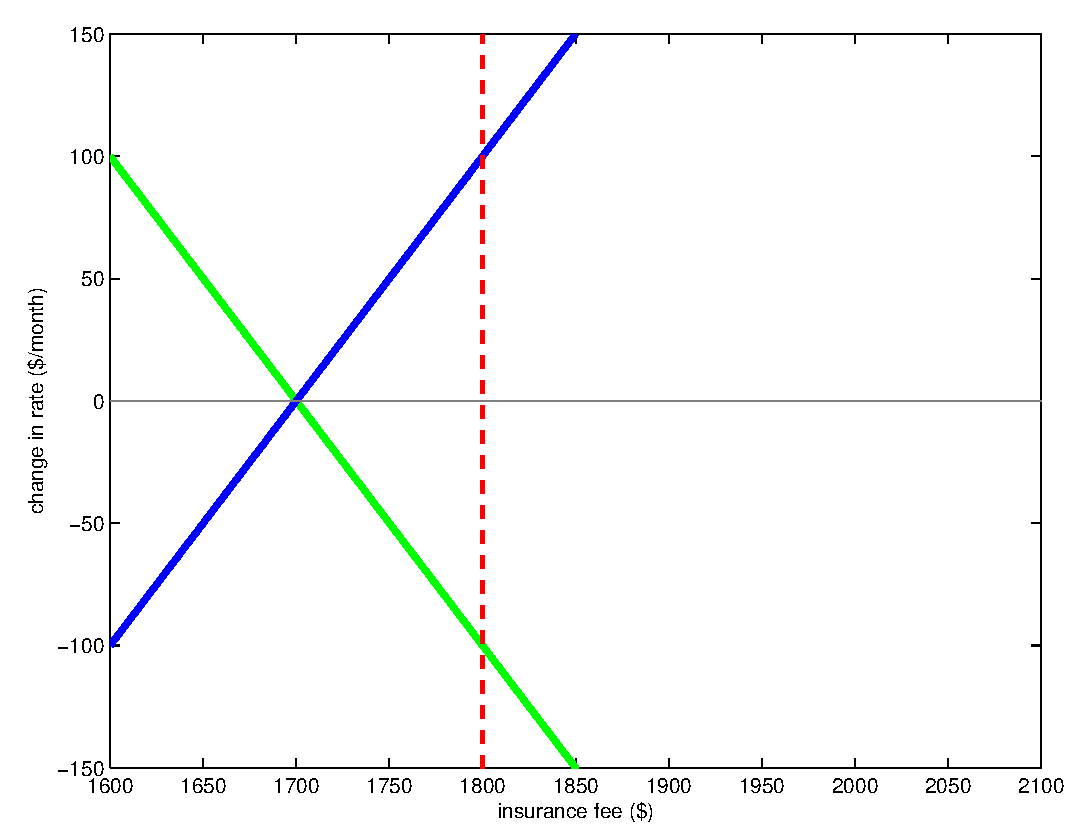
\includegraphics[width=\textwidth]{./chapter_riskless/figs/ins_lin_cropped.pdf}
\caption{Change in the rate of change of expected wealth for the shipowner (green) and the 
insurer (blue) as a function of the insurance fee, $\F$.\flabel{ins_lin}}
\end{figure}
There is no price at which the decision variable is positive for the both parties. The best they can 
do is to pick the price at which neither of them cares whether they sign or not.

In this picture, the existence of insurance contracts requires some asymmetry between the contracting parties, such as:
\begin{itemize}
\item different attitudes to bearing risk;
\item different access to information about the voyage;
\item different assessments of the riskiness of the voyage;
\item one party to deceive, coerce, or gull the other into a bad decision.
\end{itemize}
It is difficult to believe that this is truly the basis for a market of the size and global reach of the insurance market.

\subsection{Solution in the time paradigm}

\begin{example}{Time paradigm}
The insurance puzzle is resolved in the `time paradigm', \ie using 
the growth-optimal decision theory we have developed in this lecture
and multiplicative repetition. Again, we pause to reflect what multiplicative
repetition means compared to additive repetition. This is important because
additive repetition is equivalent to the expected-wealth paradigm that 
created the insurance puzzle.  Multiplicative repetition means that the 
ship owner sends out a ship and a cargo whose values are proportional to 
his wealth at the start of each voyage. A rich owner who has had many 
successful voyages will send out more cargo, a larger ship, or perhaps a \textit{flotilla}, while an owner 
to whom the sea has been a cruel mistress will send out a small vessel until his luck changes.
Under additive repetition, the ship owner would send out the same amount
of cargo on each journey, irrespective of his wealth. Shipping companies
of the size of Evergreen or Maersk would be inconceivable under additive repetition,
where returns on successful investments are not reinvested.

The two parties seek to maximise
\be
\gt_m = \lim_{\Dt\to\infty}\frac{\D\gv(\x)}{\Dt} = \frac{\ave{\d\ln \x}}{\dt},
\ee
where we have used the ergodic property of $\D\gv(\x)=\D\ln\x$
under multiplicative repetition.

The owner's time-average growth rate without insurance is 
\be
\gt_m^\text{o1} = \frac{(1-\p)\ln(\x_\text{own}+\G)+\p\ln(\x_\text{own}-\C) - \ln(\x_\text{own})}{\dt}
\ee
or 1.9\% per month. 
His time-average growth rate with insurance is 
\be
\gt_m^\text{o2} = \frac{\ln(\x_\text{own}+\G-\F)-\ln(\x_\text{own})}{\dt}
\ee
or 2.2\% per month. This gives a net benefit for the owner of
\be
\d\gt_m^o = \gt_m^\text{o1}-\gt_m^\text{o2} \approx +0.24\% \text{ per month.} 
\ee
The time paradigm thus creates a world where the owner will sign the contract.

What about the insurer? Without insurance, the insurer plays the null gamble, and
\be
\gt_m^{\text{i1}}= \frac{0}{\dt}
\ee
or 0\% per month. His time-average growth rate with insurance is 
\be
\gt_m^{\text{i2}} = \frac{(1-p)\ln(\x_\text{ins}+\F) + p\ln(\x_\text{ins}+\F-\gL) - \ln(\x_\text{ins})}{\dt}
\ee
or 0.0071\% per month. The net benefit to the insurer is therefore also
\be
\delta\gbar_m^{\text{i}} = \gt_m^{\text{i2}}-\gt_m^{\text{i1}}
\ee
\ie 0.0071\% per month. Unlike the expected wealth paradigm, the time paradigm with multiplicative repetition 
creates a world where an insurance contract can exist -- there exists a range of fees $\F$ at which
both parties gain from signing the contract! 
\end{example}


We view this as the
\begin{keypts}{Fundamental resolution of the insurance puzzle:}
The buyer and seller of an insurance contract both sign when it increases the time-average growth rates of their wealths.
\end{keypts}
It requires no appeal to arbitrary utility functions or asymmetric circumstances, rather it arises naturally from the model of human decision-making that we have set out. \fref{ins_log} shows the mutually beneficial range of insurance fees predicted by our model.
\begin{figure}
\centering
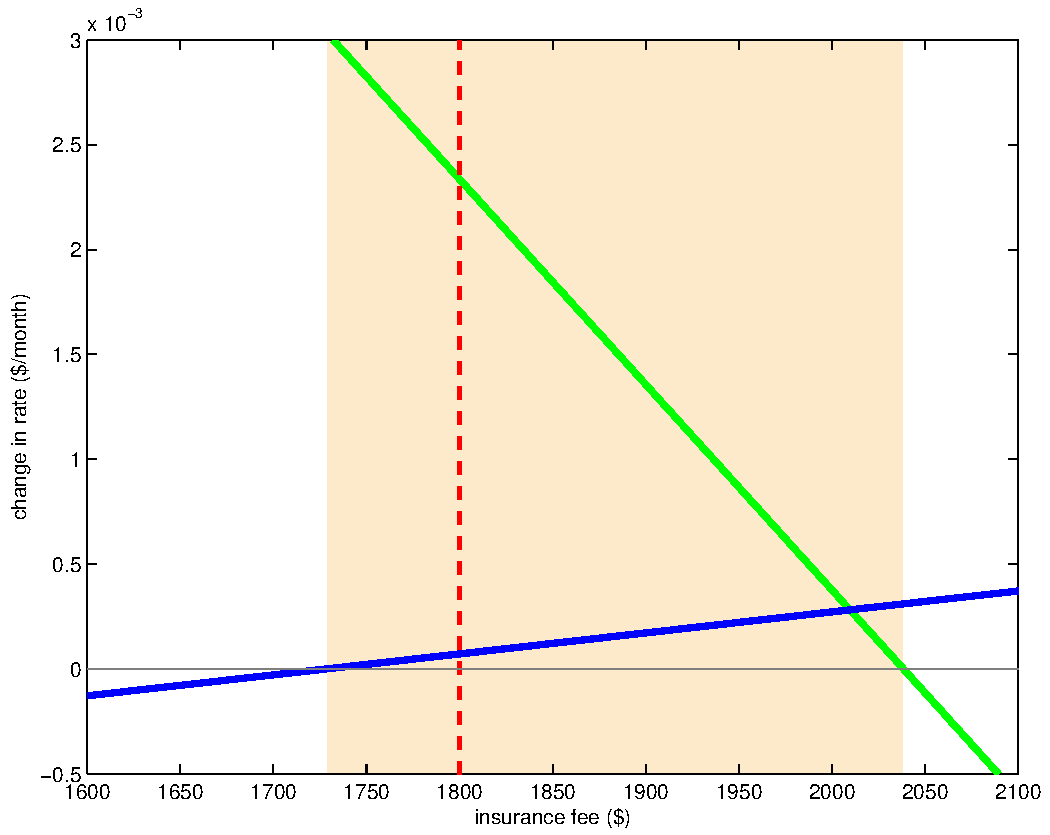
\includegraphics[width=\textwidth]{./chapter_riskless/figs/ins_log_cropped.pdf}
\caption{Change in the time-average growth rate of wealth for the shipowner (green) and the insurer (blue) as a function of the insurance fee, $F$. The mutually beneficial fee range is marked by the beige background.\flabel{ins_log}}
\end{figure}
Generalizing, the message of the time paradigm is that business happens when both parties gain.
In the world created by this model any agreement, any contract, any commercial interaction 
comes into existence because it is mutually beneficial.

%\printglossary[title=Glossary,type=\acronymtype]
%%
%\printglossary[title=List of Symbols]
\subsection{The classical solution of the insurance puzzle}
\seclabel{The classical solution of the insurance puzzle}

%\begin{example}{Expected-utility paradigm}
%Let's look at the solution in the expected-utility paradigm. Our players now seek to maximise the rate of change of their expected utility,
%\be
%\ave{r_u} \equiv \frac{\ave{\Du(W)}}{\Dt}.
%\ee
%To make the example concrete, we will use $u(W)=\sqrt{W}$, as suggested by Cramer~\cite{Cramer1728}, for both parties.
%
%The owner has
%\be
%\ave{r_u}_\text{own}^\text{un} = \frac{(1-p)u(W_\text{own}+G)+pu(W_\text{own}-C) - u(W_\text{own})}{\Dt}
%\ee
%or 3.37 `utils'\footnotemark\ per month without insurance, and 
%\be
%\ave{r_u}_\text{own}^\text{in} = \frac{u(W_\text{own}+G-F)-u(W_\text{own})}{\Dt}
%\ee
%or 3.46 utils per month with insurance. The change in $\ave{r_u}_\text{own}$ is 
%\be
%\delta\ave{r_u}_\text{own} = \ave{r_u}_\text{own}^\text{in} - \ave{r_u}_\text{own}^\text{un},
%\ee
%\ie 0.094 utils per month, and the owner should sign.
%
%The contract is also favourable from the insurer's perspective. If he does no business, then 
%\be
%\ave{r_u}_\text{ins}^\text{un} = \frac{0}{\Dt}
%\ee
%or zero utils per month. If he extends insurance, then
%\be
%\ave{r_u}_\text{ins}^\text{in} = \frac{(1-p)u(W_\text{ins}+F) + pu(W_\text{ins}+F-L) - u(W_\text{ins})}{\Dt}
%\ee
%or 0.043 utils per month and his change in $\ave{r_u}_\text{ins}$ is positive:
%\be
%\quad \delta\ave{r_u}_\text{ins} = \ave{r_u}_\text{ins}^\text{in} - \ave{r_u}_\text{ins}^\text{un},
%\ee
%\ie 0.043 utils per month.
%\end{example}
%\footnotetext{The general unit of utility. Here $1\,\text{util} = \sqrt{\$}\,1$, whatever that might mean.}
The classical solution of the insurance puzzle is identical to the classical solution of the St Petersburg paradox.
Wealth is replaced by a non-linear utility function of wealth, which breaks the symmetry of the 
expected-wealth paradigm. While it is always true that $\delta\ave{r}_\text{own}=-\delta\ave{r}_\text{ins}$, 
the expected growth rates of non-linear utility functions don't share this anti-symmetry. A difference in 
the decision makers' wealths is sufficient, though often different utility functions are assumed for owner and insurer, 
which is a model that can create pretty much any behavior. The downside of a model with this ability is, of course, 
that it makes no predictions -- nothing is ruled out, so the model cannot be falsified.
%
%This represents the classical resolution of the insurance puzzle. The symmetry broken by the different wealths $W_\text{own}$ and $W_\text{ins}$, which now appear in $\ave{r_u}$ since the utility function is nonlinear.\footnote{Note that the symmetry could also have been broken by assigning different utility functions to the two parties, even if their wealths were the same. However, it suffices only that their wealths be different for the puzzle to be resolved.} Certain combinations of $W_\text{own}$, $W_\text{ins}$, and $u$ will admit a range of mutually beneficial prices, $F$. This is visible as the beige region in \fref{ins_sqrt}, which plots the decision variable, $\delta\ave{r_u}$, for both parties as a function of the fee, $F$.
%\begin{figure}
%\centering
%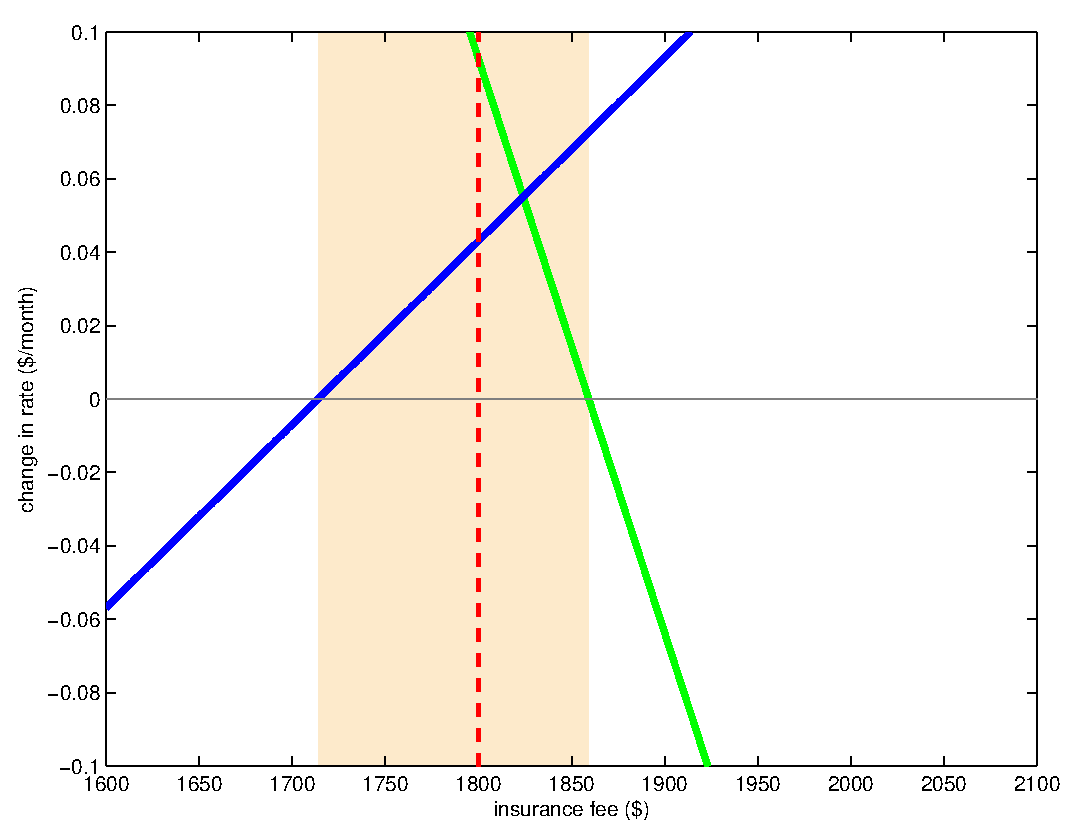
\includegraphics[width=\textwidth]{./chapter_riskless/figs/ins_sqrt_cropped.pdf}
%\caption{Change in the rate of change of expected square-root utility for the shipowner (green) and the insurer (blue) as a function of the insurance fee, $F$. The mutually beneficial fee range is marked by the beige background.\flabel{ins_sqrt}}
%\end{figure}
%Utility theory does not rule out insurance contracts -- it is {\it possible} to create a win-win deal -- but does not rule them in either. Furthermore, invoking arbitrary and unobservable utility functions hardly seems a satisfying resolution of the puzzle.